\chapter{Graphrepräsentationen von Bildern}
\label{graphrepraesentationen_von_bildern}

Als eine \emph{Graphrepräsentation eines Bildes} $\gls{B} \in {\left[0, 1\right]}^{H \times W \times C}$ wird eine Darstellung von \gls{B} als ein gewichteter, ungerichteter sowie schleifenloser Graph \gls{G} verstanden, deren Knoten Informationen zu ausgewählten Bereichen von \gls{B} über eine Merkmalsmatrix $\ma{F} \in \gls{R}^{N \times M}$ speichern und deren Kanten eine Aussage über die örtlichen Nachbarschaften eines jeden Bildbereichs inne wohnt.
Formal lässt sich eine Graphrepräsentation eines Bildes damit als ein \emph{Graph im zweidimensionalen euklidischen Raum} $\gls{G} = \left(\gls{V}, \gls{E}, \gls{p}\right)$ verstehen, dem zusätzlich zu seinen Knoten- und Kantenmengen anstatt einer Gewichtsfunktion $\gls{w} \colon \gls{E} \to \gls{R}$ eine Positionsfunktion $\gls{p} \colon \gls{V} \to \gls{R}^2$ auf seinen Knoten in den zweidimensionalen euklidischen Raum $\gls{R}^2$ zugeordnet ist.
Das Gewicht $\gls{w} \colon \gls{E} \to \left[0, 1\right]$ einer Kante ergibt sich dann als Abstandsfunktion implizit mit Hilfe der euklidischen Norm $\left\|\gls{p}\left(\gls{v}_i\right) - \gls{p}\left(\gls{v}_j\right) \right\|_2 \coloneqq \sqrt{{\left({\gls{p}\left(\gls{v}_i\right)}_1 - {\gls{p}\left(\gls{v}_j\right)}_1\right)}^2 + {\left({\gls{p}\left(\gls{v}_i\right)}_2 - {\gls{p}\left(\gls{v}_j\right)}_2\right)}^2}$ als
\begin{equation}
  \gls{w}\left(\gls{v}_i, \gls{v}_j\right) \coloneqq \begin{cases}
    \exp\left(-\frac{\left\|\gls{p}\left(\gls{v}_i\right) - \gls{p}\left(\gls{v}_j\right)\right\|_2^2}{2\gls{sigma}^2}\right), & \text{wenn }\left(\gls{v}_i, \gls{v}_j\right) \in \gls{E}\\
    0, & \text{sonst},
  \end{cases}
  \label{gauss}
\end{equation}
wobei die \emph{Gaußfunktion} $\exp\left(-x^2 / 2 \gls{sigma}^2\right)$ den Abstand zweier Knoten mit Hilfe eines festen Parameters $\gls{sigma} \in \gls{R}$ zueinander invertiert, sodass Knoten die weiter von einander entfernt liegen ein geringeres Gewicht besitzen~\cite{Shuman}.
Das korrespondiert mit der
Abbildung 5.1 veranschaulicht den Invertierungsprozess anhand unterschiedlich gewählter $\theta$.
Aufgrund der Symmetrie von ${\left\|\cdot\right\|}_2$ folgt damit sofort die Ungerichtheit des Graphen \gls{G}, \dhe{} $\gls{w}\left(\gls{v}_i, \gls{v}_j\right) = \gls{w}\left(\gls{v}_j, \gls{v}_i\right)$.

Damit lässt sich die Korrespondieren adjazenzmatrik Adist aus g() über
Zusätzlich lässt sich die Richtung der Kanten eines Graphen

Es ist insbesondere anzumerken, dass die winkelfubktion im gegensatz zur abstandsfunktion w nicht symmetrisch ist, d.h. ...
Weiterhin bildet die Winkelfunktion



Sooo
Graphen im zweidimensionalen raum
Definieren p, arad adist
Gaus

Gitter mit merkmalsfunktion f
Dann lokale oder globale normierung

Dann segmentierung


$\gls{G} = \left(\gls{V}, \gls{E}, \gls{p}\right)$

lokale oder globale Normierung

Ein \emph{ebener Graph} ist eine konkrete Darstellung eines Graphen auf der zweidimensionalen Ebene $\gls{R}^2$.
Jedem Knoten $v$ ist eine Positionsfunktion $\gls{p} \colon \gls{V} \to \gls{R}^2$ zugeordnet, die die Position eines Knotens auf der Ebene eindeutig definiert.

\gls{Adist} und \gls{Arad} machen Graphen translationsinvariant und abhängig von Sigma auch skalierungsinvariant


\section{Gitter}
\label{gitter}

Die einfachste Form einer Graphrepräsentation \gls{G} eines Bildes $\gls{B} \in \gls{R}^{H \times W \times C}$ ist die Repräsentation des Bildes über einen regulären Gittergraphen, denn dafür müssen keine Berechnungen am Bild vorgenommen werden.
Ein \emph{regulärer Gittergraph im zweidimensionalen euklidischen Raum} ist ein Graph $\gls{G} = \left(\gls{V}, \gls{E}, \gls{p}\right)$, der aus einem regulären Gitter gewonnen wurde und demnach genau $N \coloneqq H \times W$ Knoten enthält, \dhe{} einen Knoten für jedes Pixel in \gls{B}~\cite{Defferrard}.
Die Positionsfunktion der Knoten $\gls{p} \colon \gls{V} \to \gls{R}^2$ entspricht damit genau der Koordinate des korrespondierenden Pixels im Urpsprungsbild.
Sei dafür $\gls{v} \in \gls{V}$ der Knoten zu dem Bildpunkt an Position $\left(x,y\right)$.
Folglich gilt für die Position des Knotens $\gls{p}\left(\gls{v}\right) \coloneqq {\left[x,y\right]}^{\top}$.
Die örtlich um den Knoten $\gls{v} \in \gls{V}$ liegenden Knoten gelten dann auch im Gittergraph als benachbart und werden über eine Kante in \gls{E} verbunden.
Dabei unterscheidet man zwischen zwei frei wählbaren \emph{Konnektivitäten} des Graphen~\cite{Defferrard}.
Eine Konnektivität von $4$ bedeutet, dass ein Knoten (ohne Berücksichtigung der Randknoten) genau vier Nachbarn besitzt, die horizontal und vertikal zu im stehen.
Bei einer Konnektivität von $8$ gelten zusätzlich die vier diagonal zu ihm stehenden Knoten als Nachbarn und die Nachbarschaft wird folglich als ein $3 \times 3$ Fenster um den Knoten \gls{v} verstanden.

Analog zu den Daten der Farbkanäle an den einzelnen Pixeln des Bildes hängt auch an den Knoten über einer Merkmalsfunktion $f \colon \gls{V} \to \gls{R}^C$ \bzw{} einer Merkmalsmatrix $\ma{F} \in \gls{R}^{N \times C}$ diese Information mit $f\left(\gls{v}\right) \coloneqq \gls{B}_{{p\left(\gls{v}\right)}_2,{p\left(\gls{v}\right)}_1}$.

\paragraph{Effiziente Adjazenzbestimmung}
\label{adjazenzbestimmung_gitter}

Entgegen der Pixelanordnung in einem Bild ist die Anordnung der Knoten in einem Gittergraphen völlig irrelevant und kann willkürlich gewählt werden.
Ein Aufbau der Kantenmenge \gls{E} \bzw{} der korrespondierenden, ungewichteten Adjazenzmatrix \gls{A} kann jedoch besonders effizient gestaltet werden, wenn die Knoten reihenweise entsprechend ihrer Bildkoordinate angeordnet werden.
Dafür wird das Bild \gls{B} zunächst an dessen Rändern um eine zusätzliche Spalte \bzw{} Reihe erweitert, \dhe{} $\gls{B} \in {\left[0, 1\right]}^{\left(H + 2\right) \times \left(W + 2\right) \times C}$.
Dann besitzt die ungewichtete Adjazenzmatrix $\gls{A} \in {\left\{0, 1\right\}}^{N \times N}$ mit $N \coloneqq \left(H+2\right)\left(W+2\right)$ in den Reihen $W+3 < i < N - W - 3$ an den Spaltenindizes $\left\{i-W-2, i-1, i+1, i+W+2\right\}$ \bzw{}
\begin{equation*}
  \left\{i-W-3, i-W-2, i-W-1, i-1, i+1, i+W+1, i+W+2, i+W+3\right\}
\end{equation*}
genau einen Eintrag gleich Eins (bei einer Konnektivität von $4$ \bzw{} $8$).
Anschließend müssen die ungültigen Knoten aus \gls{A} reihen- und spaltenweise schrittweise über eine Länge von $W$ mit Schrittweite $W+2$ gefiltert werden.
Dabei müssen natürlich zunächst die ersten und letzten $W + 3$ Knoten aus \gls{A} gelöscht werden.

\begin{figure}[t]
\centering
\subfigure[\gls{SLIC}]{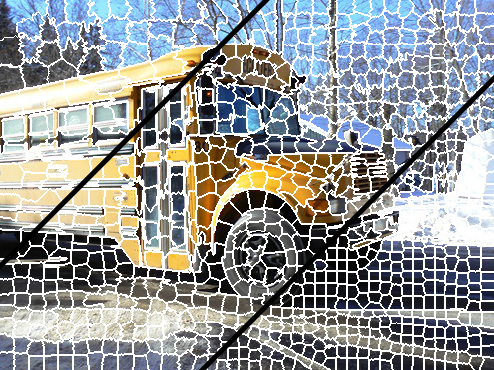
\includegraphics[scale=0.4]{bilder/slic_beispiel}}
\subfigure[Quickshift]{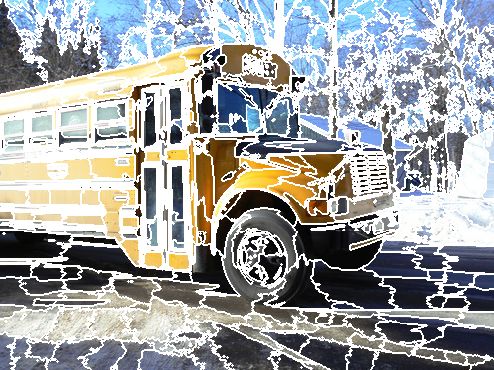
\includegraphics[scale=0.4]{bilder/quickshift_beispiel}}
  \caption[\gls{SLIC} und Quickshift Beispielresultat]{Ein Bus segmentiert über \gls{SLIC} mit jeweils 400, 800 und 1600 Superpixeln (a) sowie über Quickshift mit 600 Superpixeln (b).
  Dabei werden die unterschiedlichen Verfahren zur Generierung von Superpixeln deutlich.
  Wohingegen \gls{SLIC} möglichst quadratische, gleichgroße Superpixel erzeugt, wird die Form der Superpixel von Quickshift größtenteils über die Farbabgrenzungen gesteuert und erzeugt damit sowohl sehr große wie auch sehr kleine Superpixel in allen möglichen Variationen.}
\label{fig:slic_quickshift}
\end{figure}

